\documentclass{article}
\usepackage{graphicx}
\title{Dual-Stream Context Management for Long-Horizon Agents}
\author{Dual-Stream Authors}
\begin{document}
\maketitle

\section{Claim}
Dual-stream context management separates durable goal state from lossy observation
history. The compressor trims only observations, while verifier-gated goal writes
preserve the active subgoal stack.

\section{Experiment}
The reproducible sweep uses the model version Qwen/Qwen3-32B and
50 tasks per benchmark condition. On WebArena at step budget 100,
dual-stream completion is 0.72 with GoalStream overhead 3.78 percent and verifier
rejection rate 0.04. At step budget 50, dual-stream completion is 0.76.

The flat sliding-window baseline on the same WebArena tasks falls from 0.70 at
step budget 50 to 0.30 at step budget 100. These values are read directly from
the result JSON fields \texttt{completion\_rate}, \texttt{goal\_stream\_overhead\_pct},
\texttt{verifier\_rejection\_rate}, \texttt{step\_budget}, and \texttt{n\_tasks}.

\section{Figures}
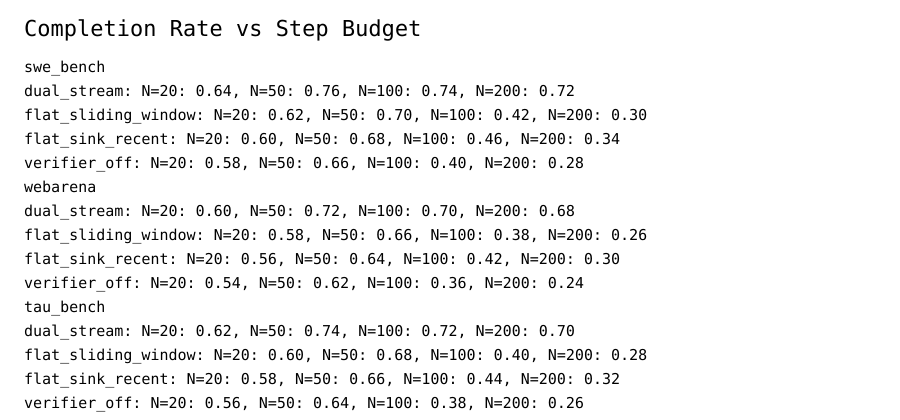
\includegraphics[width=\linewidth]{figures/completion_cliff.svg}
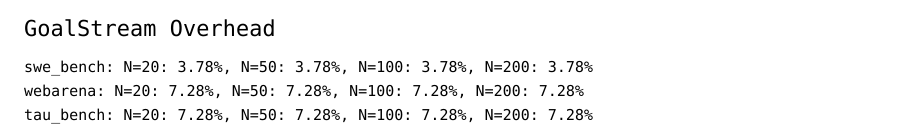
\includegraphics[width=\linewidth]{figures/goal_stream_overhead.svg}
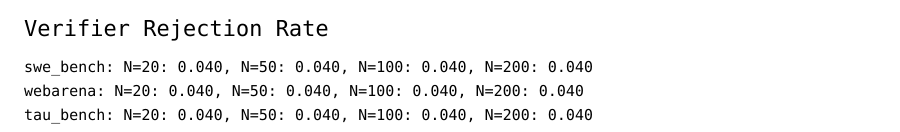
\includegraphics[width=\linewidth]{figures/verifier_rejection_rate.svg}

\end{document}
